\chapter{Introduction}
For the mini project in the Robot Vision 2018 course the task of assembling Simpsons figures with a robot was given. The figures are made of \lego Duplo bricks stacked on each other as can be seen in \autoref{fig:Simpsons_duplo}. The figures are the following:

\begin{itemize}
\item Homer: Yellow, Red, Blue
\item Bart: Yellow, Orange, Blue
\item Maggie: Yellow, Red
\item Lisa: Yellow, Orange, Yellow
\item Marge: Blue, Yellow, Green
\end{itemize}

\begin{figure}[h]
\centering
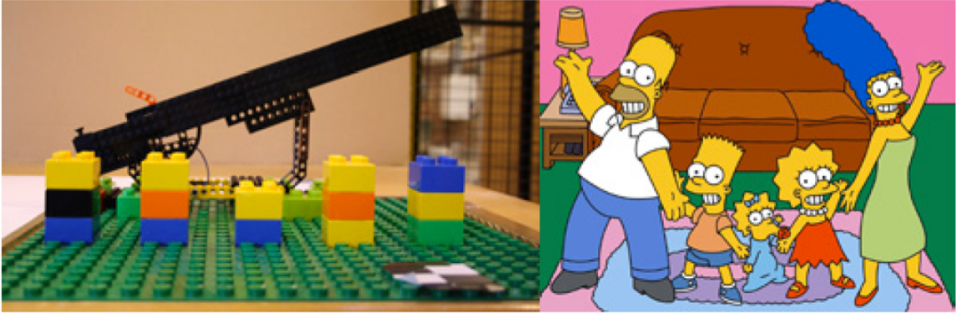
\includegraphics[width=\textwidth]{figures/simpsons_duplo_figures.png}
\caption{}
\label{fig:Simpsons_duplo}
\end{figure}

To automatically solve this task a robot and a camera is needed in a setup like \autoref{fig:robot_theoretical_setup}. The camera takes pictures of the area where the bricks are located. The image is then processed to figure out where the bricks are located and how they are oriented. The robot is then ordered to assemble a figure e.g. Homer and can now do this automatically since it knows where the bricks are. The figure is then assembled and dropped off in a loading area and the robot prepares for a new order. 

\begin{figure}[h]
\centering
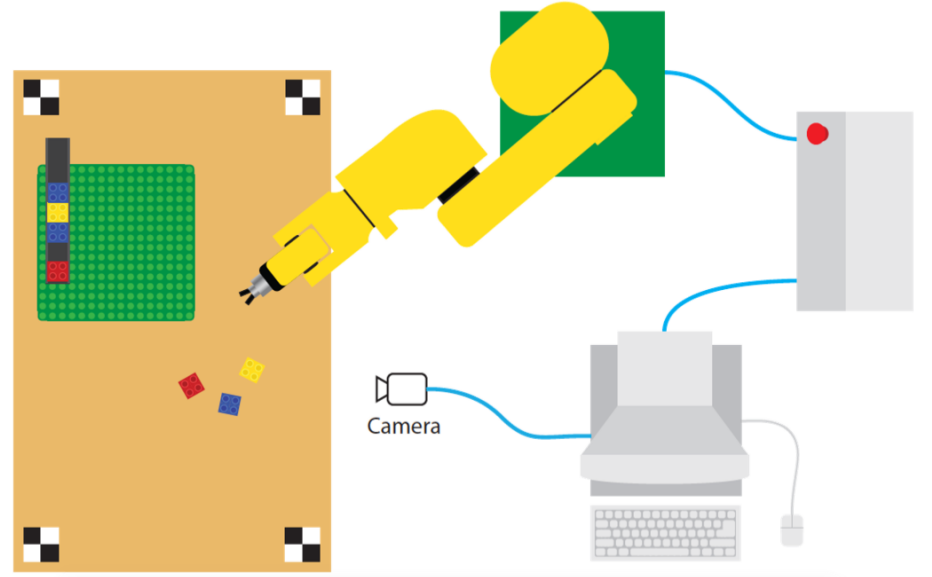
\includegraphics[width=\textwidth]{figures/robot_theoretical_setup.png}
\caption{}
\label{fig:robot_theoretical_setup}
\end{figure}